\documentclass[12pt,liststotoc]{report}
\usepackage[T1]{fontenc}
\usepackage[utf8x]{inputenc}
\usepackage{color}
\usepackage{geometry}
\geometry{a4paper, top=30mm, left=30mm, right=30mm, bottom=30mm, headsep=10mm, footskip=12mm} 
\usepackage{amsfonts}
\usepackage{amsmath}
\usepackage[ngerman]{babel}
\usepackage{graphicx}
\usepackage{booktabs}
\usepackage{tabularx}
\usepackage{array}
\usepackage{textcomp}
\usepackage{amssymb}
\usepackage{amstext}
\usepackage{subfigure}
\usepackage{amsfonts}
\usepackage{mathrsfs}
\usepackage{csquotes}
\usepackage{multirow}
\usepackage{color}
\usepackage{bigstrut}
\usepackage[version=4]{mhchem}
\usepackage{textcomp} 
\usepackage{nicefrac}
\usepackage{caption}
\usepackage{lmodern}
\usepackage{pdflscape}
\usepackage{pdfpages}
\usepackage{here} 
\newcommand{\rtab}{\raggedleft\arraybackslash}

\usepackage{hyperref}
\usepackage{fancyref}
\usepackage{todonotes}
\usepackage{bigints}
\usepackage{amsmath}
\usepackage{amssymb}
\usepackage{amstext}
\usepackage{amsfonts}
\usepackage{mathrsfs}
\usepackage[version-1-compatibility]{siunitx}

%\usepackage[backend=biber,style=alphabetic,sorting=ynt]{biblatex}
%\addbibresource{Quelle_CRT_2.bib} 
 



\usepackage{ngerman}
\setlength{\parindent}{0em}	
\setlength{\parskip}{1.5ex plus0.5ex minus0.5ex}

\usepackage{chemformula}

\captionsetup[table]{skip=5pt}


\begin{document}
\setcounter{secnumdepth}{5}
\setcounter{tocdepth}{5}

\begin{titlepage}
	\centering
	
\includegraphics[width=0.5\textwidth]{Graphics/TU_Graz.pdf}\par\vspace{1cm}
	
	{\scshape\LARGE Reaktionstechnik II LU  \par}
	\vspace{1cm}
	{\scshape\Large LU 667.212\par}
	{\scshape \large SS 2018\par}
	\vspace{0.5cm}
	{\huge\bfseries Verweilzeitverteilung\par}
	\vspace{0.5cm}

	{\LARGE \itshape Ashok Andermann\par}
	{\large 11729115\par}\vspace{0.5cm}
	%\vspace{0,2cm}	
	
	{\LARGE \itshape Kilian Fleisch\par}
	{\large 11744809\par}\vspace{0.5cm}
	%\vspace{0,2cm}
	
		
	{\LARGE \itshape Jakob Geistlinger\par}
	{\large 01131349\par}\vspace{0.5cm}
	%\vspace{0,2cm}
	
	{\LARGE \itshape Felix Lechleitner\par}
	{\large 01316701\par}\vspace{0.5cm}
	%\vspace{0,2cm}

	{\LARGE \itshape Tobias Maier\par}
	{\large 01330853\par}\vspace{0.5cm}
	%\vspace{0,2cm}
	\vfill

% Bottom of the page
	{\large \today\par}
\end{titlepage}


\pagenumbering{Roman}
\tableofcontents
\newpage
\pagenumbering{arabic}
\chapter{Einleitung \& Aufgabenstellung}

\cite{Dean_Wirbel}; \cite{Rolfe1934}; \cite{Skript_2018}, \cite{fogler1999elements}; \cite{mandake2013kinetic}; \cite{Chem_Reaktion_2018}, \cite{Skript_CVT_MCI}}

\par Rohrreaktoren werden in der Industrie häufig eingesetzt, z.B. für die Synthese von Polyamid bzw. allgemein für Polymerisationsreaktionen. \cite{fogler1999elements}, \cite{Chemgapedia}
Um große Volumina erreichen zu können werden Rohrbündelreaktoren aus mehreren einzelnen Rohrreaktoren verwendet. Im Rahmen dieses Experiments werden die realen Verweilzeitverteilungen von zwei Kunststoffrohrreaktoren aus REHAU-rauclair-e $\copyright$ mit und ohne Füllkörpern verglichen, wobei die Füllkörper Glaskugeln mit Durchmesser $\approx$ 1\,mm sind. 
\\
\\
Basierend darauf sollten theoretische Vergleiche mit verschiedenen idealen Reaktoren angestellt und die Effekte auf eine hypothetisch darin ablaufende Reaktion diskutiert werden. Dazu wird einerseits die Stoß- und andererseits die Sprungfunktion analysiert, wobei als Tracer eine NaCl-Lösung verwendet wird. In weiterer Folge kann die Altersverteilung und die kumulative Verteilung ermittelt werden um daraus die mittlere Verweilzeit, Varianz und verschiedene Vergleiche mit dem Dispersions- und Kaskadenmodell anzustellen. Des Weiteren kann der Einfluss der Verweilzeitverteilung auf eine hypothetisch im Reaktor ablaufende Reaktion diskutiert werden.


%\par Ziel dieser Laborübung war die Bestimmung der Verweilzeitverteilung zweier Rohrreaktoren.
%Basierend darauf sollten theoretische Vergleiche mit verschiedenen idealen Reaktoren angestellt und die Effekte auf eine hypothetisch darin ablaufende Reaktion diskutiert werden.

%\par Die Verweilzeitverteilung wurde jeweils durch eine Stoßfunktion sowie eine Sprungfunktion experimentell ermittelt. Daraus wurde die mittlere Verweilzeit und die Varianz berechnet, und die Daten mit idealen Reaktoren Verglichen. 



\chapter{Versuchsaufbau}


Als Fluid ohne Tracer ($H_2O$) wird nicht reines deionisiertes verwendet aber mit Leitungswasser vermischt um eine Grundleitfähigkeit zu erhalten. Deionisiertes Wasser wird mit Leitungswasser vermischt damit immer eine Grundleitfähigkeit vorhanden ist, reines deionisiertes Wasser hätte ebenfalls eine Leitfähigkeit die nicht bei 0 liegt sondern ca. 50\,$\mu$S/cm \cite{Leitfahigkeit_Wasser}, aber um eine Grundleitfähigkeit sicherzustellen wird Leitungswasser hinzugegeben. Wäre der Wert der Leitfähigkeit $\kappa$ gleich 0 ergeben sich mit der gewählten Berechnungsmethode für $E(t)$ Werte gegen $\infty$.

%\begin{figure}[H]
%\centering
%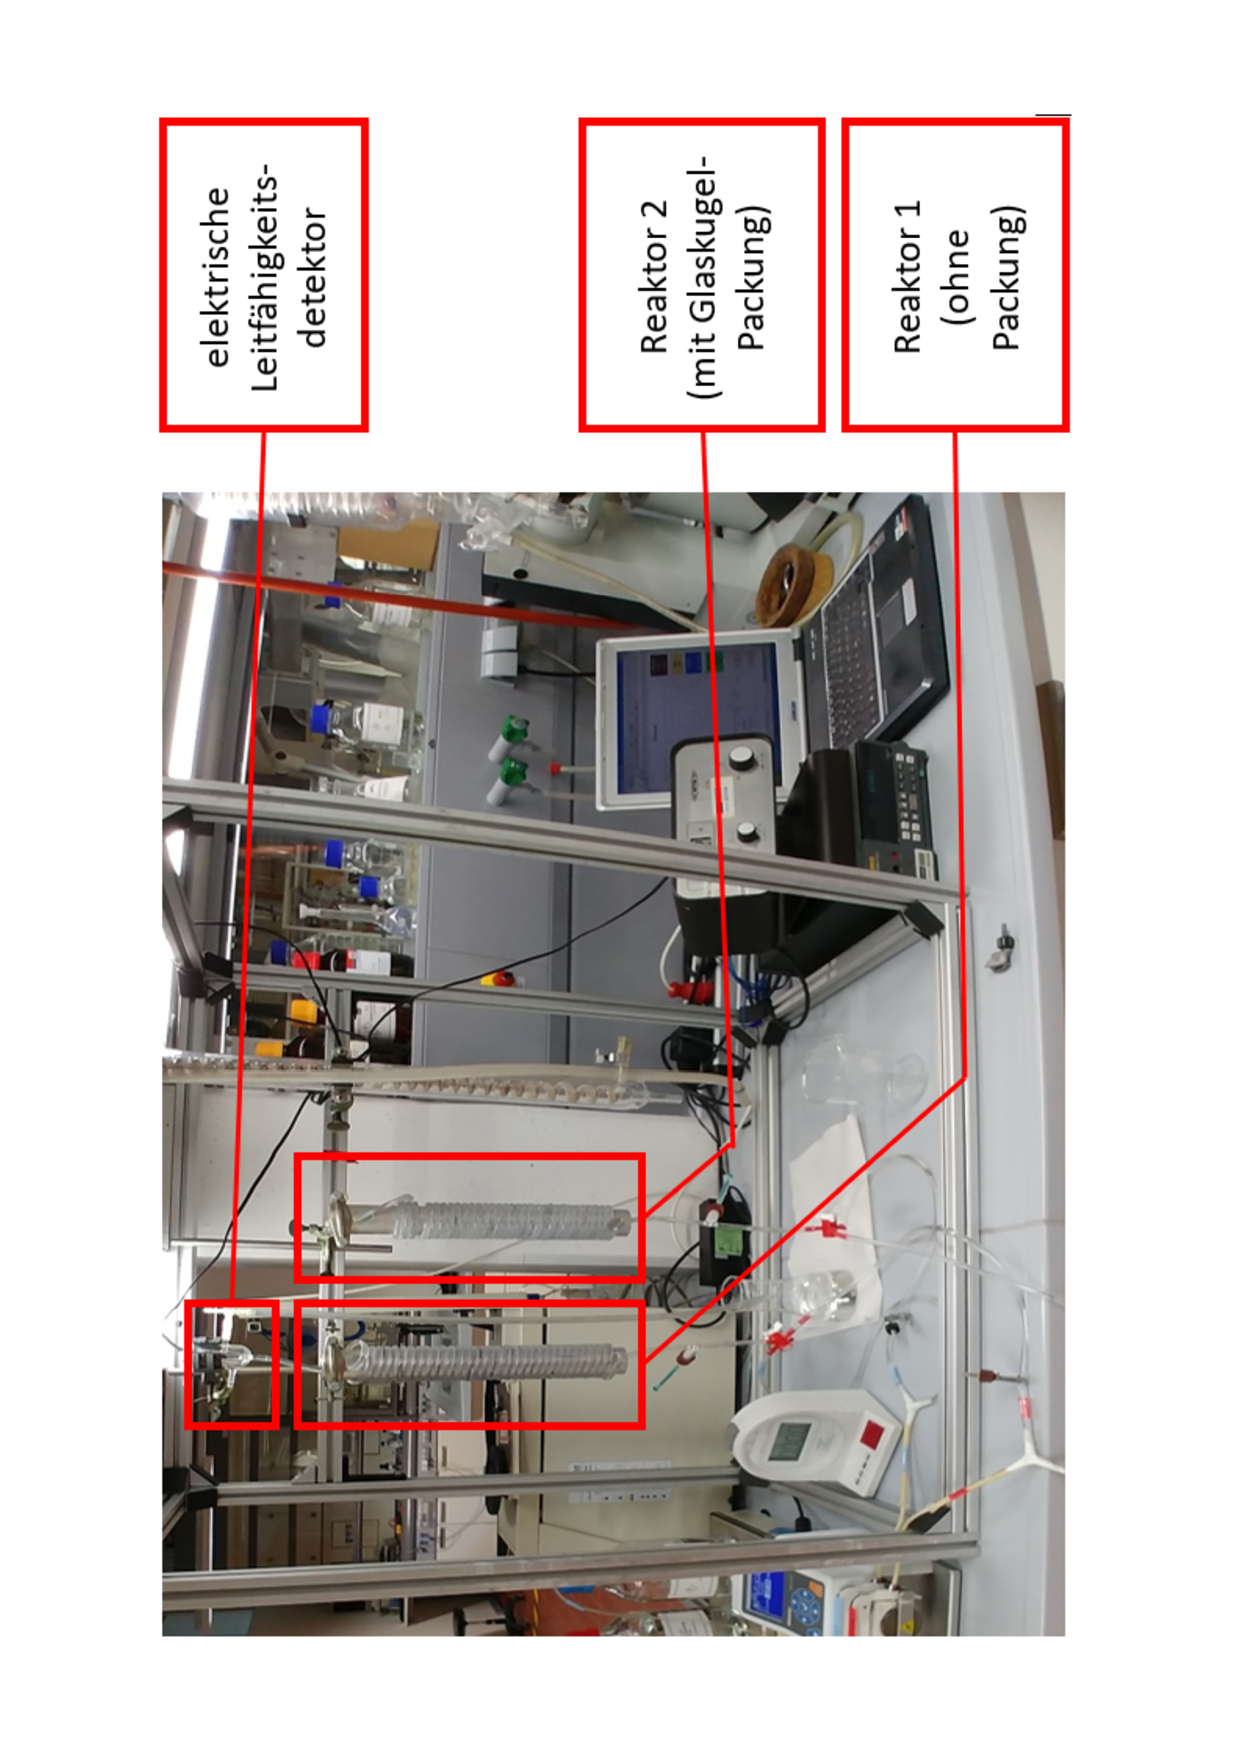
\includegraphics[angle=270,width=0.8\textwidth]{Graphics/Versuchsaufbau.pdf} 
%\caption{Versuchsaufbau [1] (Skript Labor)}
%\label{Versuchsaufbau}
%\end{figure}
%\noindent

Der Versuchsaufbau besteht aus zwei verschiedenen „plug-flow-reactors“ (PFRs), einer Schlauchquetsch-Pumpe, zwei Lagertanks, einer mit H$_2$O und einer mit in Wasser gelösten NaCl (Marker / Tracer), einem Chronometer und einer Leitfähigkeitszelle. Der gesamte Aufbau ist in Abbildung \ref{Versuchsaufbau} dargestellt.
Die beiden Reaktoren sind als 5\,m lange Kunststoffrohre mit einem Durchmesser von 5\,mm ausgeführt, die auf einem Metallrohr aufgewickelt sind. Ein Reaktor ist mit Glaskugeln gefüllt, während der andere keine Packung aufweist. Der Aufbau des Experiments ist in Abbildung \ref{Versuchsaufbau} zu sehen. Abbildung \ref{Prozessfliessbild} zeigt das Prozessfließbild des Versuchs. Am Ende der beiden Reaktoren befindet sich Leitfähigkeitsdetektor, der die Konzentration an Tracer bestimmt.

\begin{figure}[H]
\centering
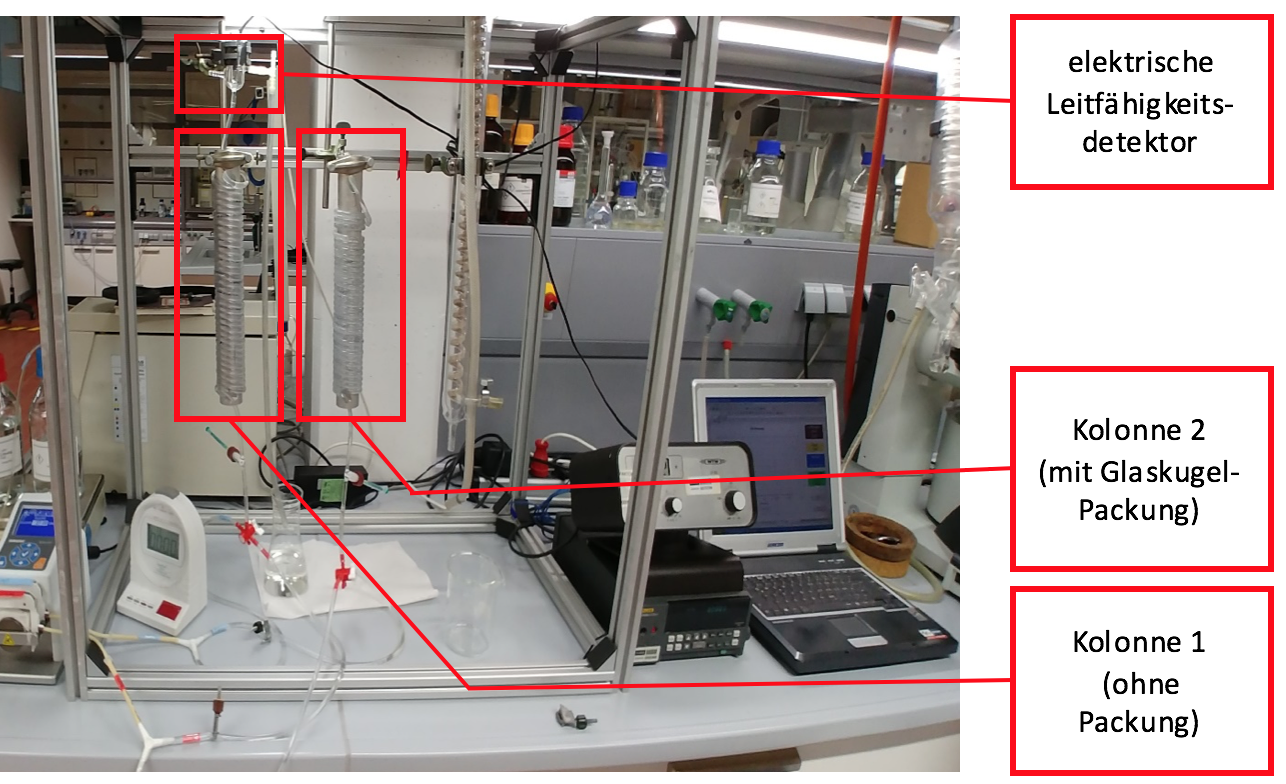
\includegraphics[width=0.8\textwidth]{Graphics/Versuchsaufbau.png} 
\caption[Versuchsaufbau des Experiments zur Bestimmung der Verweilzeitverteilung zweier PFRs mit NaCl als Tracer]{Versuchsaufbau des Experiments zur Bestimmung der Verweilzeitverteilung zweier PFRs mit NaCl als Tracer \cite{Skript_2018}}
\label{Versuchsaufbau}
\end{figure}
\noindent

\begin{figure}[H]
\centering
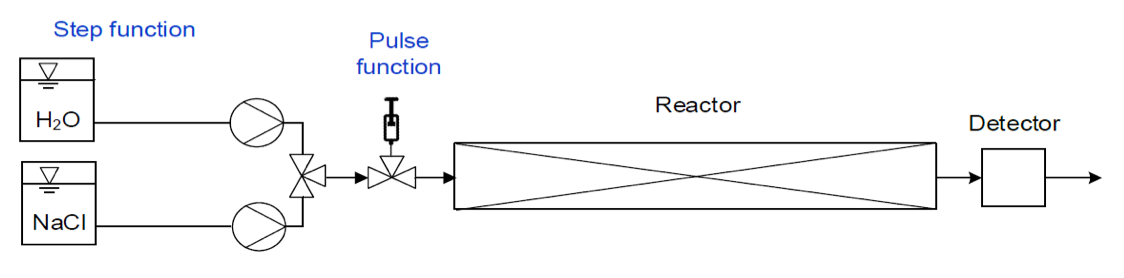
\includegraphics[width=0.8\textwidth]{Graphics/Prozessfliessbild.png} 
\caption[Prozessfliessbild des Versuchs]{Prozessfliessbild des Versuchs \cite{Skript_2018}}
\label{Prozessfliessbild}
\end{figure}
\noindent






\chapter{Durchführung}

%Zu Beginn wird eine Kalibrationskurve der Schlauchquetschpumpe erstellt. Dazu wird die Zeit gemessen, welche benötigt wird um eine bestimmte Masse zu fördern, in diesem Falle 5\,g. 


Vor Beginn der Versuche muss eine Kalibration der Schlauchquetsch-Pumpe durchgeführt werden, um den genauen Durchfluss der Pumpe zu bestimmen. Dabei wird das Gewicht des Fluiddurchsatzes nach einer gewissen Zeit gemessen. Die Menge wird durch die Zeit geteilt, um einen Wert für die Durchflussrate zu ermitteln. In Tabelle \ref{tab:Pumpenkalibration} sind die Ergebnisse der Pumpenkalibration dargestellt. Über die Dichte wird der gemessene Massenstrom in den Volumenstrom übergeführt, wobei zur Ermittlung der Pumpenkennlinie eine Dichte von reinem Wasser mit $\rho_{H_2O}$= 1000\,$\frac{\text{kg}}{\text{m}^3}$ herangezogen wird.

\begin{gather*}
\dot{m} = \frac{m}{\Delta t} \\
\\
\dot{V} = \dot{m} \cdot \rho
\end{gather*}
\\
\\
Nach der Kalibration der Pumpe können die Versuche durchgeführt werden. Zwei verschiedene Injektionsarten (Impulsfunktionen und Schrittfunktionen) werden verwendet. Für die Versuche werden drei unterschiedliche Volumenströme im Reaktor gewählt. Tabelle \ref{tab:Volumenströme} zeigt die Umdrehungszahlen der Pumpe für die verschiedenen Durchsätze, die für beide Reaktoren gleich sind.
\\
\\
In den Pulsfunktionsexperimenten wird der Reaktor mit deionisiertem Wasser betrieben und der Tracer wird über eine kurze Zeit (fast sofort) über eine Spritze injiziert. Bei der Injektion ist unbedingt darauf zu achten, dass der Auslass der Spritze in Strömungsrichtung zeigt, um das Strömungsverhalten möglichst wenig zu beeinflussen. Abbildung \ref{Injektionsvorrichtung} zeigt die Strömungsrichtung und die Injektionsvorrichtung für die Pulsfunktion. Das Experiment gilt als abgeschlossen, sobald die Konzentration des Tracers am Ausgang des Reaktors gegen Null geht bzw. die „Startkonzentration“ wieder erreicht wird.

\begin{figure}[H]
\centering
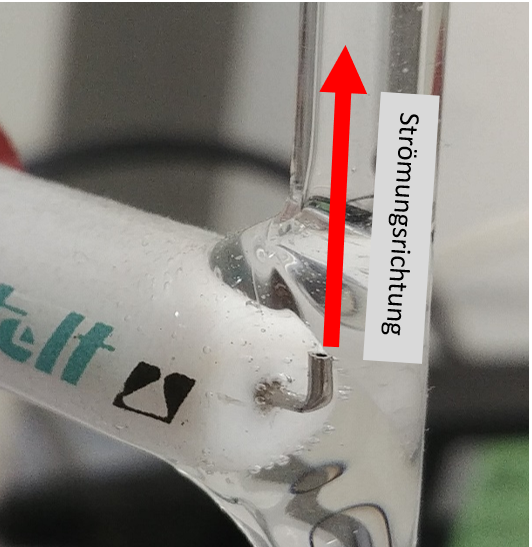
\includegraphics[width=0.5\textwidth]{Graphics/Injektionsvorrichtung.PNG}
\caption{Injektionsvorrichtung für die Pulsfunktion}
\label{Injektionsvorrichtung}
\end{figure}
\noindent
In den Stufenfunktionsversuchen wird der Reaktor zunächst mit deionisiertem Wasser betrieben und am Startpunkt wird das Dreiwegeventil geschaltet, um das Wasser mit dem Tracer nun kontinuierlich durch den Reaktor zu transportieren. Das Experiment gilt als abgeschlossen, sobald die Konzentration des Tracers am Ausgang des Reaktors ca. konstant ist. 

\begin{table}[H]
\centering
\caption[Pumpenkalibration]{Die Zeit um 5\,g an deionisiertem Wasser zu transportieren wird bei verschiedenen Umdrehungszahlen der Pumpe gemessen, um die Durchflussrate zu bestimmen}
\begin{tabular}{ccc}
\toprule 
Drehzahl in $\frac{1}{\text{min}}$ & Zeit in s & Durchfluss in $\frac{\text{g}}{\text{min}}$\\
\midrule
10 & 119 & 2,52\\
20 & 78 & 3,85 \\
30 & 56 & 5,36 \\
40 & 30 & 10,00 \\
50 & 24 & 12,50 \\
\bottomrule
\end{tabular}
\label{tab:Pumpenkalibration}
\end{table}
\noindent

\begin{table}[H]
\centering
\caption{Umdrehungen pro Minute der Pumpe für die Volumenströme der Versuche}
\begin{tabular}{cc}
\toprule 
Drehzahl in $\frac{1}{\text{min}}$ & Volumenstrom in $\frac{\text{ml}}{\text{min}}$\\
\midrule
27 & 7 \\
38 & 10 \\
49 & 13 \\
\bottomrule
\end{tabular}
\label{tab:Volumenströme}
\end{table}
\noindent



\chapter{Ergebnisse $\&$ Interpretation}

\section{Bestimmung der Verweilzeitverteilung für Stoß- und Pulsfunktion}


   
 %  \missingfigure{Versuche deklarieren, Versuch 1-3 im Reaktor 1 \& Versuch 1-3 im Reaktor 2, dass referenziert werden kann}

Aus den detektierten Werten, welche die Leitfähigkeit der verwendeten NaCl-Lösung darstellen, kann mittels der Kohlrauschfunktion [Quelle] in die Konzentration umgerechnet werden. In den weiterführenden Berechnungen wird die Konzentration verwendet. Die Berechnung der Konzentration ist Beispielhaft für xy durchgeführt:



\begin{figure}[H]
\centering
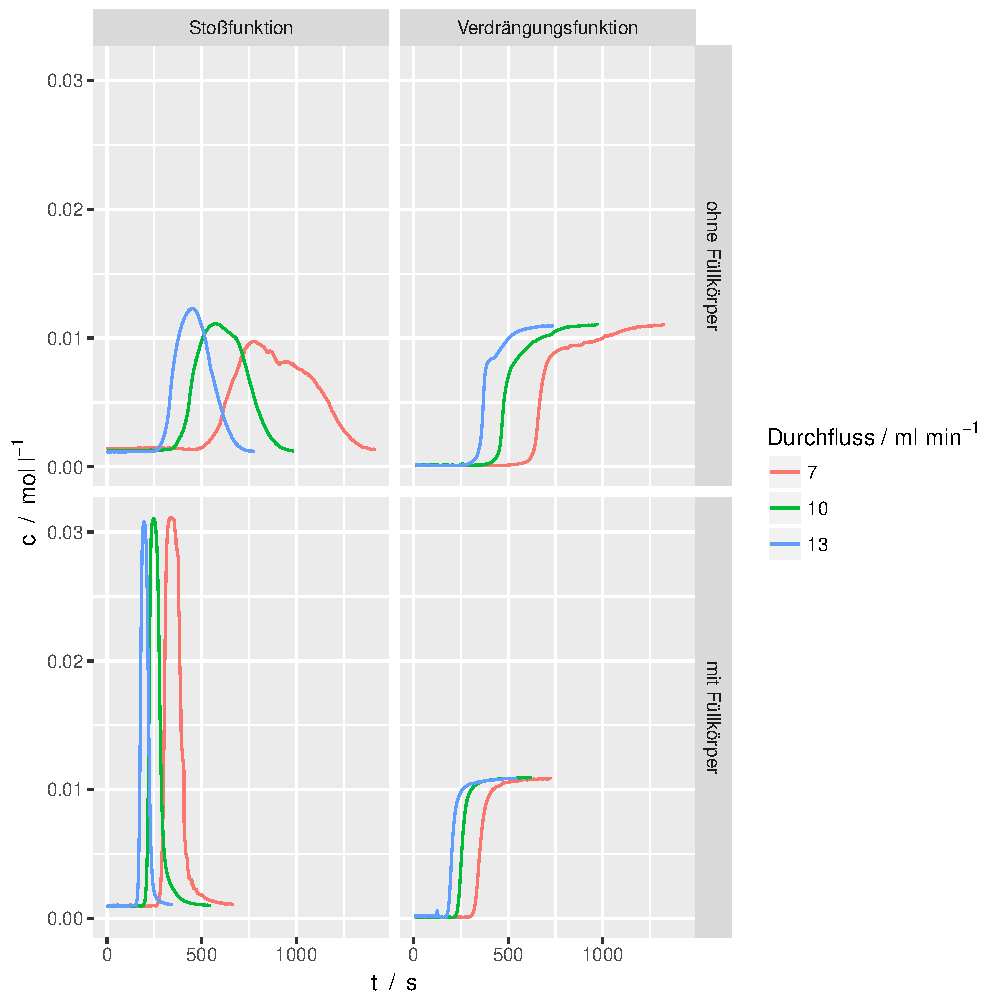
\includegraphics[width=1\textwidth]{Graphics/ct.pdf}
\caption[Konzentrationsverläufe]{Konzentrationsverläufe der einzelnen Versuche}
\label{konzentrationsverlauf}
\end{figure}
\noindent
Im weiteren Verlauf der Darstellung der Ergebnisse werden die Versuche numeriert um eine einfachere Zuweisung zu ermöglich. Diese Numerierung ist in Tabelle \ref{tab:Versuchsnummerierung} dargelegt.

\begin{table}[H]
\centering
\caption{Versuchsnummerierung}
\begin{tabular}{c|c|c|cc}
\toprule 
Versuchsnummer $\#$ & Reaktor & Volumenstrom in $\frac{\text{ml}}{\text{min}}$ & Experiment \\
\midrule
1 & ohne Füllk.& 7 & Puls \\
2 & ohne Füllk. & 10 & Puls \\
3 & ohne Füllk. & 13 & Puls \\
4 & mit Füllk. & 7 & Puls \\
5 & mit Füllk. & 10 & Puls \\
6 & mit Füllk. & 13 & Puls \\
7 & ohne Füllk. & 7 & Stufen \\
8 & ohne Füllk. & 10 & Stufen \\
9 & ohne Füllk. & 13 & Stufen \\
10 & mit Füllk. & 7 & Stufen\\
11 & mit Füllk. & 10 & Stufen \\
12 & mit Füllk. & 13 & Stufen\\
\bottomrule
\end{tabular}
\label{tab:Versuchsnummerierung}
\end{table}
\noindent


\section{Stoßmarkierung}

Im Rahmen der Ermittlung der Verweilzeitverteilung mittels der Stoßmarkierung werden ca. 0,4\,ml einer NaCl-Lösung mit einer Spritze in den Rohrreaktor an einer Stelle zwischen der Schlauchquetschpumpe, welche weiterhin das Gemisch aus demineralisiertem H$_2$O und Leitugnswasser fördert, und dem aufgewickelten Rohr, injiziert. Damit sollte im Idealfall am Ausgang des Reaktors an der Messstelle ein starkes Signal in einem engen Zeitintervall gemessen werden. Im realen Fall ist das Signal aber über einen längeren Zeitraum detektierbar und muss daher über die gemessene Leitfähigkeit bzw. die daraus resultierende Konzentration beschrieben werden. Die dazu notwendigen Gleichungen beziehen sich auf Quelle [Skript].
 
\subsection{Verweilzeitdichtefunktion E(t) aus Stoßmarkierung}

Das Ergebnis der Stoßmarkierung ist ein Peak im Konzentrations-Zeit-Diagramm. Dieser Peak wird in die sogenannte Verweilzeitdichteverteilung umgerechnet. Das Integral dieser Kurve, sprich die Flächte unter der Kurve, entspricht dem Wert 1. Bei Diskretisierung der Zeitschritte lässt sich die Summe numerisch generieren. Die Verweilzeitdichteverteilung ist wie folgt charakterisiert:


\begin{align}
E(t) =&\;\frac{c_{i}}{\int_{0}^{\infty} c_{i}\cdot \text{d}t_i}\,\approx\,\frac{c_i}{\sum c_i \cdot \Delta t_i}\\
\textit{mit }\sum c_i \cdot \Delta t_i =&\; c_1\cdot\Delta t_1 + c_2\cdot\Delta t_2 +\;...\;+c_n \cdot \Delta t_n \\
\sum c_i \cdot \Delta t_i =&\; 0,0014\,\frac{\mole}{\litre} \cdot 3\,\s + 0,0015\,\frac{\mole}{\litre}\cdot 3\,\s +\;...\notag\\
&...\;+0,0013\,\frac{\mole}{\litre} \cdot 3\,\s \approx 5,9118\,\frac{\mole\cdot\s}{\litre}\notag\\\notag
\end{align}

Für die beispielhafte Konzentration von $0,0090\,\mole\cdot\litre^{-1}$ bei Sekunde 864 ($\Delta t = 3\,\s$) ergibt sich folgender Wert für die Funktion $E(t)$:

\begin{equation*}
E(864\,\s) = \frac{0,0091\,\frac{\mole}{\litre}}{5,9118\,\frac{\,\mole\cdot\s}{\litre}} \approx0,0015\,\frac{1}{\s}
\end{equation*}

Mit Hilfe der Progammiersprache \textit{'"R'"} werden die im Laufe des Versuchs generierten Werte aus \textit{Excel} zu den jeweiligen Zeitpunkten eingelesen und es werden nach obigem Rechenschema die dazugehörigen Werte für die Verweilzeitdichtefunktion kalkuliert. Die Start- und End-Zeitpunkte für die jeweiligen Versuche werden händisch laut den dokumentierten Werten eingelesen. Die weiteren Berechnungen  werden ebenfalls mit dieser Datenauswertungsmethode durchgeführt.

\begin{figure}[H]
\centering
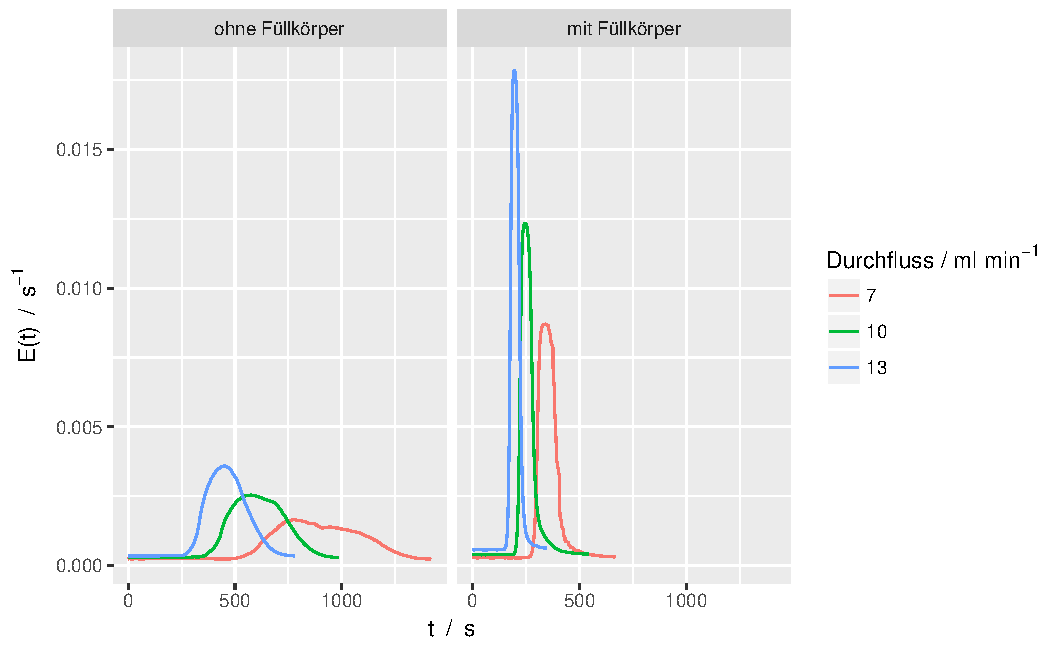
\includegraphics[width=1\textwidth]{Graphics/E_stoss.pdf}
\caption[Verweilzeitdichte Stoßmarkierungen]{Verweilzeitdichten aus der Stoßmarkierung}
\label{dichte_stoß}
\end{figure}
\noindent

%Die Software erzeugt zudem die Diagramme, welche später angeführt werden.

\subsection{Verweilzeitsummenfunktion F(t)}

Aus der Verweilzeitdichtefunktion kann durch das Integral in Abhängigkeit der Zeit die Verweilzeitsummenfunktion generiert werden. Die Funktion F(t) ist eine prozentuelle Angabe und hat ihr Maximum demnach bei 1, ist einheitenlos und beschreibt die Zeitspanne in welcher der gesamte Tracer den Ausgang des Reaktors passiert hat bzw. das Maximum, sprich die Konzentration der zugeführten Lösung, gemessen wird. Bei numerischer Lösung des Integrals wird folgende Gleichung für die Berechnung der Summenfunktion angewandt:

\begin{align}
F(t) =&\; \int_{0}^{t} E(t_i) \cdot \text{d} t_i \approx \sum E(t_i) \cdot \Delta t_i\\
F(t_n) =&\;E(t_1) \cdot \Delta t_1 + E(t_2) \cdot \Delta t_2+\;...\;+E(t_n) \cdot \Delta t_n\\\notag
\end{align}

Für 553\,s ergibt sich folgender Wert:

\begin{equation*}
F(553\,\s) =0,0002\,\frac{1}{\s}\cdot 3\,\s + 0,0001\,\frac{1}{\s}\cdot3\,\s+\;...\;+ 0,0008\,\frac{1}{\s} \cdot 3\,\s \approx 0,9585
\end{equation*} 

\begin{figure}[H]
\centering
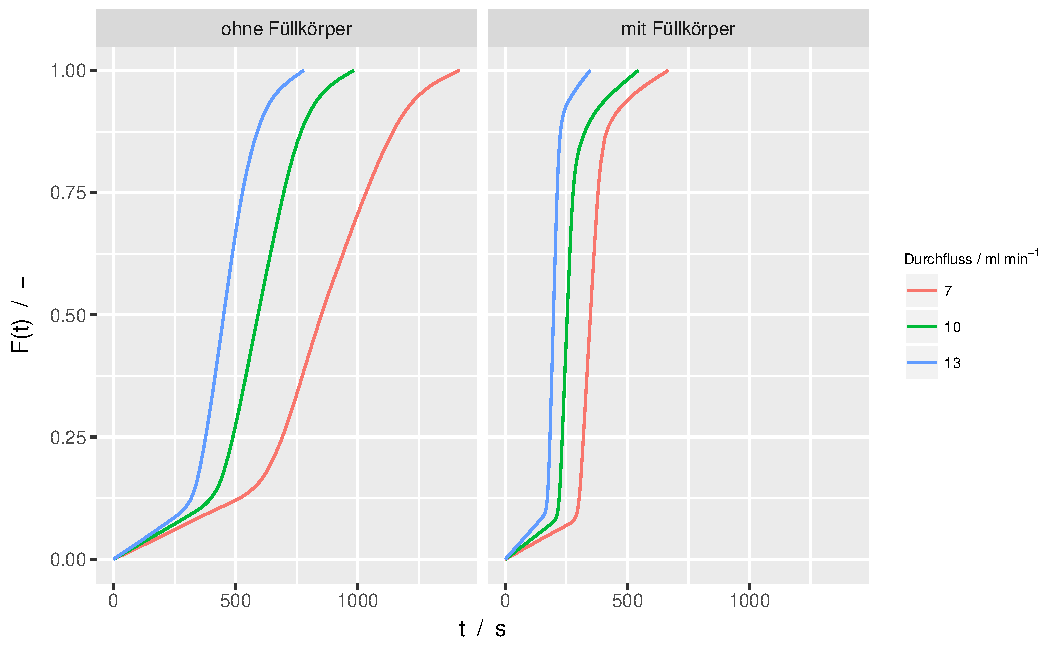
\includegraphics[width=1\textwidth]{Graphics/F_stoss.pdf}
\caption[Verweilzeitsumme Stoßmarkierungen]{Verweilzeitsummen aus der Stoßmarkierung}
\label{summe_stoß}
\end{figure}
\noindent

\subsection{Normierte Verweilzeitdichtefunktion $E(\theta)$}

Unter Einbindung der dimensionslosen Verweilzeit $\theta$ bzw. der mittleren Verweilzeit $\bar{t}$ kann die normierte Verweilzeitsummenfunktion bestimmt werden. Die Integrale der mittleren Verweilzeit können ebenfalls diskretisiert ausgedrückt werden. Die Berechnung ist im Folgenden dargestellt:

\begin{align}
E(\theta_i) =&\; E(t_i) \cdot \bar{t} \\
\text{mit }\theta_i=&\;\frac{t_i}{\bar{t}}\\
\text{und }\bar{t} = &\;\frac{\int_{0}^{\infty}t_i\cdot c_i \cdot\text{d}t_i}{\int_{0}^{\infty}c_i \cdot\text{d}t_i} \approx \frac{\sum t_i\cdot c_i \cdot \Delta t_i}{\sum c_i \cdot \Delta t_i}\\ 
\end{align} 

Die Summe von $\sum c_i \cdot \Delta t_i$ wurde zuvor berechnet. Für $\sum t_i\cdot c_i \cdot \Delta t_i$ ergibt sich für der unten berechnete Wert. Des Weiteren lässt sich anschließend $\bar{t}$ und $E(\theta)$ ($t= 640\,s$) für den ersten Versuch im ersten Reaktor berechnen:

\begin{align*}
\sum t_i\cdot c_i \cdot \Delta t_i =&\;t_1\cdot c_1 \cdot \Delta t_1 + t_2\cdot c_2 \cdot \Delta t_2+\;...\,+t_n\cdot c_n \cdot \Delta t_n \\
\sum t_i\cdot c_i \cdot \Delta t_i =&\; 3\,\s\cdot 0,0014\,\frac{\mole}{\litre}\cdot 3\,\s + 6\,\s\cdot 0,0015\,\frac{\mole}{\litre}\cdot 3\,\s+\;...\\
&...\;+ 1416\,\s\cdot 0,0013\,\frac{\mole}{\litre}\cdot 3\s \approx 4912,0634\,\frac{\mole\cdot\s^2}{\litre}\\
\bar{t} =&\; \frac{4912,0634\,\frac{\mole\cdot\s^2}{\litre}}{5,9118\,\frac{\mole\cdot\s}{\litre}} \approx 830,89\,\s\\
E(\theta_{640\,\s}) =&\; E(640\,\s)\cdot\bar{t} = 0,0010\,\frac{1}{\s} \cdot 830,89\,\s \approx 0,7992\\
\end{align*} 


\begin{figure}[H]
\centering
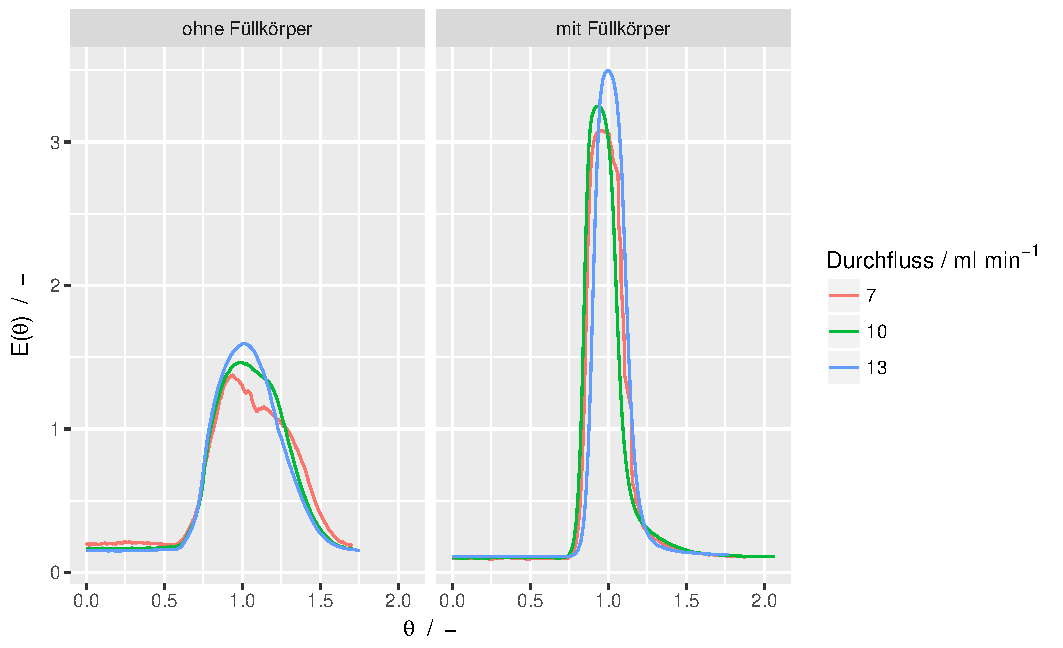
\includegraphics[width=1\textwidth]{Graphics/E_theta_stoss.pdf}
\caption[normierte Verweilzeitdichte Stoßmarkierungen]{normierte Verweilzeitdichten aus der Stoßmarkierung}
\label{dichte_stoß_norm}
\end{figure}
\noindent


Die Verläufe der einzelnen Kurven für alle Versuche sind im Folgenden in Abbildungen XXX-XXX ersichtlich. 


\subsection{Berechnung der Standardabweichung und des Dispersionsgrades $\sigma^{2}_{t}$, $\sigma_\theta$, Bo}

Letztendlich lässt sich aus allen Informationen, die durch den Versuch generiert werden können, die Standardabweichung $\sigma^{2}_t$, standardisierte Standardabweichung $\sigma^{2}_\theta$ und die Bodenstein-Zahl $Bo$ errechnen, welche ein Maß für die Dispersion und somit axiale Rückvermischung im betreffenden Reaktor ist. Durch Diskretisierung kann das Integral abermals numerisch gelöst werden:

\begin{align}
\sigma^{2}_t =&\;\frac{\int_{0}^{\infty}(t_i-\bar{t})^2\cdot c_i \cdot\Delta t_i}{\int_{0}^{\infty}c_i\cdot\Delta t_i} \approx \frac{\sum t_{i}^2\cdot c_i \cdot\Delta t_i}{\sum c_i\cdot\Delta t_i} - \bar{t}^2\\
\sigma_\theta^2 =&\;\frac{\sigma^{2}_t}{\bar{t}^2}\\
\text{Bo} =&\; \frac{2}{\sigma_\theta^2}\\
\text{mit } \sum t_{i}^2\cdot c_i \cdot\Delta t_i =&\; t_{1}^2\cdot c_1 \cdot\Delta t_1 + t_{2}^2\cdot c_2 \cdot\Delta t_2+\;...\;+t_{n}^2\cdot c_n \cdot\Delta t_n\\
\sum t_{i}^2\cdot c_i \cdot\Delta t_i =&\; 9\,\s^2\cdot 0,0014\,\frac{\mole}{\litre} \cdot 3\,\s + 36\,\s^2\cdot 0,0015\frac{\mole}{\litre} \cdot \s+\;...\nonumber\\\notag
&...\;+ 2005056\;\s^2\cdot 0,0013\;\frac{\mole}{\litre} \cdot 3\;\s \approx 4580895,1998\,\frac{\mole \cdot \s^3}{\litre}\notag
\end{align}

Für die Parameter errechnet sich:

\begin{align*}
\sigma^{2}_t =&\;\frac{ 4580895,1998\,\frac{\mole \cdot \s^3}{\litre}}{ 4912,0634\frac{\mole \cdot \s}{\litre}} - 690373,4860
\,s^2\approx 774038,3948
s^2\\
\sigma_\theta^2 =&\; 774038,3948\,\frac{\s^2}{690373,4860\,\s^2}\approx 1,1212\\
\text{Bo} =&\; \frac{2}{1,1212}\approx 1,7849
\end{align*}

\todo{fertig machen, wenn Delta t weg dann funktionierts ansonsten passts nicht, passt was nicht}

\section{Verdrängungsmarkierung}


\subsection{Verweilzeitsummenfunktion F(t)}

Das Ergebnis der Verdrängungsmarkierung liefert eine S- bzw. Sigmoidale- Kurve im Konzentrations-Zeit-Diagramm. Diese Kurve wird in die Verweilzeitsummenverteilung zur Interpretation des Verweilzeitverhalten des Reaktors umgerechnet, wobei es an dieser Stelle wichtig ist zu erwähnen, dass für weitere Berechnungen die Fläche der Kurve im Unterschied zur Stoßfunktion bzw. Stoßmarkierung seitlich nach links und nicht unter der Kurve integriert wird. Sie beschreibt den Anteil der Konzentration, die gemessen wird, im Verhältnis zur effektiven maximalen Konzentration. Die maximale Konzentration ergibt sich aus den Messungen. Sobald sich eine stationäre Konzentration einstellt, wird der Versuch beendet. Diese stationäre Konzentration kann somit als $c_{max}$ definiert werden. 

\begin{align}
F(t_i)=&\;\frac{c_i(t_i)}{\Delta c_{max}}\\
\text{mit } \Delta c_{max} =&\; c_{max} - c_{min}\\
\text{bzw. wenn } c_{min} =&\; 0 \text{ dann } \Delta c_{max} = c_{max} 
\end{align}

Für die Abbildung der Verweilzeitsummenverteilung müssen anschließend die einzelnen Werte für $F(t)$ addiert werden. Für die 332 Sekunde ergibt sich beispielsweise:

\begin{equation}
F(332\,s)=\,...+\,\frac{ 0,0008\,\frac{\mole}{\litre}}{ 0,0110\,\frac{\mole}{\litre}} \approx 0,0724 \notag
\end{equation}

\todo{passt nich mit dem Diagramm überein}

\begin{figure}[H]
\centering
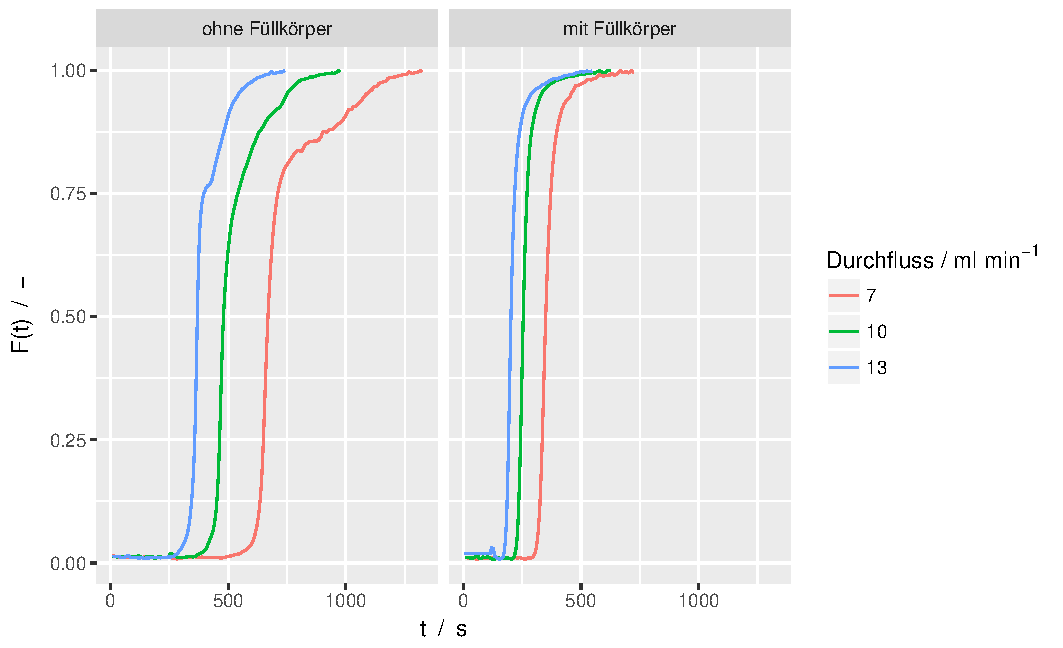
\includegraphics[width=1\textwidth]{Graphics/F_step.pdf}
\caption[Verweilzeitsumme Sprungfunktion]{Verweilzeitsummen aus der Sprungfunktion}
\label{summe_step}
\end{figure}
\noindent

\subsection{Verweilzeitdichteverteilung E(t)}

Die Verweilzeitdichteverteilung kann durch Ableiten der Verweilzeitsummenverteilung kalkuliert werden. Unter Anwendung diskreter Zeitschritte $\Delta t$ und Werten für $\Delta F (t)$ ergeben sich folgende Werte:

\begin{align}
E(t_i)=&\; \frac{\Delta F(t_i)}{\Delta t_i}= \frac{F(t_{i})-F(t_{i-1})}{t_i-t_{i-1}}\\
E(332\,\s)=&\; \frac{0,0724
 - 0,0651}{332\,\s - 229\,\s} = 0,0024
\,\frac{1}{s}\notag
\end{align}

\begin{figure}[H]
\centering
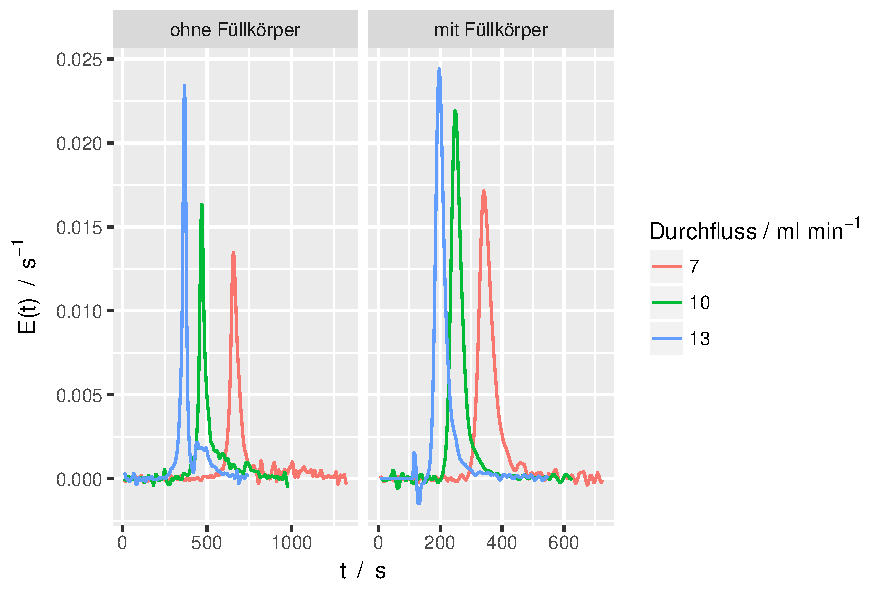
\includegraphics[width=1\textwidth]{Graphics/E_step.pdf}
\caption[Verweilzeitdichte Sprungfunktion]{Verweilzeitdichten aus der Sprungfunktion}
\label{dichte_step}
\end{figure}
\noindent

\subsection{Normierte Verweilzeitdichteverteilung $E(\theta)$}

Die Berechnung der standardisierten Verweilzeitdichteverteilung läuft analog zur Stoßverteilung ab. Lediglich die mittlere Verweilzeit errechnet sich durch eine andere Gleichung. Die Gleichung lässt sich wie folgt darstellen:

\begin{align}
\bar{t}=&\; \frac{\int_{0}^{c_{max}}t_i \cdot\text{d}c_i}{\int_{0}^{c_{max}}\text{d}c_i}\approx \frac{\sum t_i\cdot\Delta c_i}{\Delta c_{max}}\\
\sum t_i\cdot\Delta c_i =&\; t_1\cdot\Delta c_1 + t_2\cdot\Delta c_2+\;...\;+t_n\cdot\Delta c_n\\
\sum t_i\cdot\Delta c_i =&\; 9\,\s\cdot0,0001\,\frac{\mole}{\litre}  + 12\,\s\cdot 0,0000\,\frac{\mole}{\litre}+\;...\notag\\
&...\;+757\,\s\cdot (-0,0020)\,\frac{\mole}{\litre}\approx 2,8082\,\frac{\mole\cdot\s}{\litre} \notag
\end{align}

Für den ersten Versuch aus dem ersten Reaktor ohne Füllkörper ergibt sich folgende mittlere Verweilzeit:

\begin{equation}
\bar{t}= \frac{2,8082\,\frac{\mole\cdot\s}{\litre}}{0,0110\,\frac{\mole}{\litre}} \approx 255,2909\,\s\notag
\end{equation}

\begin{figure}[H]
\centering
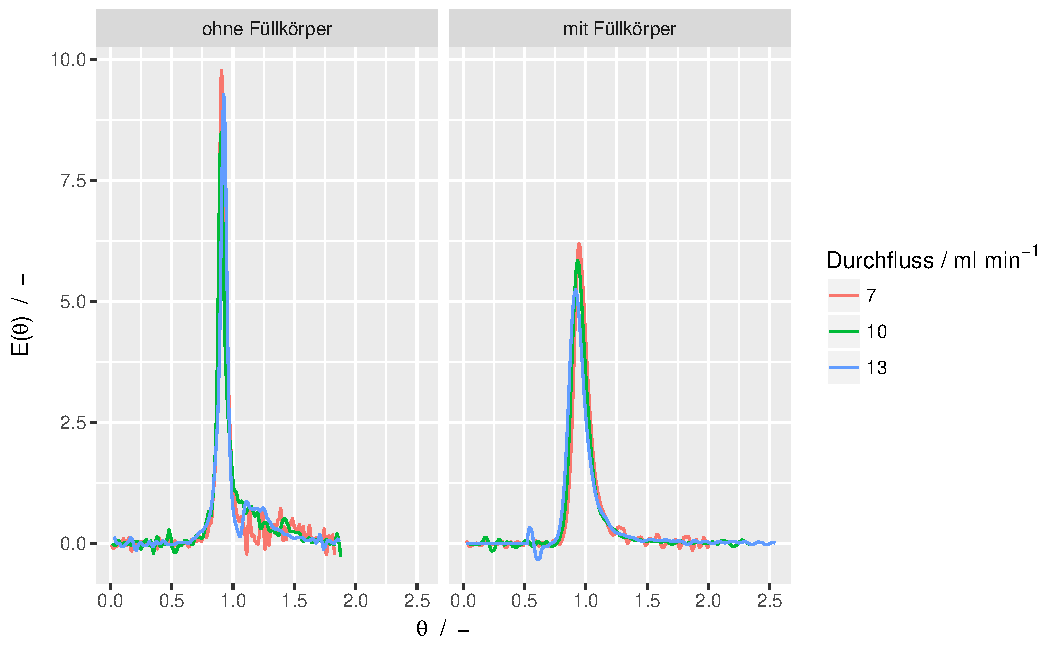
\includegraphics[width=1\textwidth]{Graphics/E_theta_step.pdf}
\caption[normierte Verweilzeitdichte Sprungfunktion]{normierte Verweilzeitdichten aus der Sprungfunktion}
\label{dichte_step_norm}
\end{figure}
\noindent



\subsection{Berechnung der Standardabweichung und des Dispersionsgrades $\sigma^2$}

Die Bodenstein-Zahl und $\sigma_\theta^2$ errechnen sich simultan zu Punkt xy. Zuvor wird $\sigma_t^2$ nach folgendem Schema errechnet: 
 
\begin{align}
\sigma_t^2=&\;\frac{\sum t_i^2\cdot\Delta c_i}{\Delta c_{max}} - \bar{t}^2\\
\text{mit } \sum t_i^2\cdot\Delta c_i =&\;t_1^2\cdot \Delta c_1 + t_2^2\cdot \Delta c_2 +\;...\;+t_n^2\cdot \Delta c_n\\
 \sum t_i^2\cdot\Delta c_i =&\;81\,\s^2 \cdot 0,0001\,\frac{\mole}{\litre} + 144\,\s^2 \cdot 0,0000\,\frac{\mole}{\litre}+\;...\notag\\\notag
&...\;+ 573049\, \s^2 \cdot (-0,0020)\frac{\mole}{\litre}\approx 628,1782\,\frac{\mole\cdot\s^2}{\litre}\\\notag
 \sigma_t^2=&\;\frac{628,1782\,\frac{\mole\cdot \s^2}{\litre}}{0,0110\,\frac{\mole}{\litre}} - 65173,4483\,\s^2 \approx 56949,7365\,\s^2\\\notag
\end{align}

\todo{stimmt auch nicht ganz}

\section{Vergleich der experimentell ermittelten Verteilungen}

Vergleiche und Abweichungen



\section{Beschreibung der Verweilzeitsummenfunktion mit dem Kaskadenmodell}


Ein Rohrreaktor verhält sich im idealen Fall wie eine Rührkesselkaskade, sprich eine Serienschaltung von Rührkesseln mit der Anazhl an Rührkesseln $N$. Geht die Anzahl der Rührkessel gegen unendlich $N \rightarrow \infty$ ist das Verhalten eines idealen Rohrreaktors ersichtlich. Im realen Fall wird daher das ideale Strömungsrohr durch eine bestimmte Anzahl an Rührkesseln angenähert. Im Folgenden wird die Verweilzeitsummenfunktion für alle Versuche aus dem Kaskadenmodell generiert. Die äquivalente Anzahl an Rührkesseln nach dem Kaskadenmodell wird über $E_{\theta,max}$ laut [Skript] berechnet. $E_{\theta,max}$ wird aus der erzeugten Kurve ausgelesen oder über die Bodenstein-Zahl berechnet:

\begin{align}
&N = -1,762 + 0,569\cdot E_{\theta,max} + 6,206\cdot (E_{\theta,max})^2\\
&E_{\theta,max}=\biggl(\frac{4\cdot\pi}{\text{Bo}}\biggl)^{-0,5} = E_{\theta,max}=\biggl(\frac{4\cdot\pi}{\text{Bo}}\biggl)^{-0,5} \approx 
\end{align}

Für $E_{\theta,max}$ nach dem grafischen Ablesen ergibt sich xy. Nach der Berechnung mit einer Bodenstein-Zahl von xy ergibt sich $E_{\theta,max}$ von. Im Folgenden sind beide Berechnungen für $N_1$ und $N_2$ ersichtlich:

\begin{align*}
&N_1 = -1,762 + 0,569\cdot E_{\theta,max} + 6,206\cdot (E_{\theta,max})^2\approx \text{Rührkessel}\\
&N_2 = -1,762 + 0,569\cdot E_{\theta,max} + 6,206\cdot (E_{\theta,max})^2\approx  \text{Rührkessel}\\
\end{align*}

Anschließend wird nach dem Kaskadenmodell die Verweilzeitsummenverteilung für eine Anzahl von $N$ Rührkesseln erzeugt. Dabei genügt F(t) im Kaskadenmodell dem folgenden Modell:

\begin{align}
c_{i,N}^{aus}=c_{i,N}^{ein} \cdot &\Biggl(1-\text{e}^{-N\cdot\frac{t}{\tau}} \cdot \biggl(1+2\cdot\frac{t}{\tau} + \frac{1}{2!}\cdot \Bigl(3\cdot\frac{t}{\tau}\Bigr)^2 +\;...\\
&...\;+\frac{1}{(N-1)!}\cdot\Bigl(N\cdot\frac{t}{\tau}\Bigr)^{N-1} \biggr)\Biggr) \nonumber\\\notag 
&\text{wobei } \frac{c_{i,N}^{aus}}{c_{i,N}^{ein}}= \frac{c_i(t_i)}{c_{max}}=F(t_i)\\\notag
&\text{und } \tau = \bar{t}\notag
\end{align}

Damit ergibt sich für eine Anzahl von N=14 Rührkessel folgender Wert bei t s

\begin{align}
F(t)=&\Biggl(1-\text{e}^{-14\cdot\frac{\s}{\s}} \cdot \biggl(1+2\cdot\frac{\s}{\s} + \frac{1}{2!}\cdot \Bigl(3\cdot\frac{\s}{\s}\Bigr)^2 +\;...\\
&...\;+\frac{1}{(14)!}\cdot\Bigl(15\cdot\frac{\s}{\s}\Bigr)^{14} \biggr)\Biggr)\approx \nonumber
\end{align}

\begin{align}
F(t) = \Biggl(1-\text{e}^{-14 \cdot \frac{t}{\bar{t}}} \cdot \biggl(1+2\cdot \frac{t}{\bar{t}} + \frac{1}{2!} \cdot \Bigl(
\end{align}

Wird nun aus der Summenverteilung die Dichtverteilung gebildet (siehe Kapitel xy) und anschließend eine neue Kurve für $E(\theta)$ erzeugt, kann ein neues $E_{\theta,max}$ abgelesen bzw. bestimmt werden. Dies liefert eine neue Anazhl an Rührkesseln und weiters eine neue Summenverteilung. Durch dieses iterative Vorgehen wird die Kurve angenähert und die optimale Anzahl an $N$ ermittelt, welche das reale Strömungsrohr am Besten beschreibt. Die Ergebnisse dieses Vorgehens sind im Folgenden in Tabelle XXX und Abbildungen XXX-XXX dokumentiert bzw. zusammengefasst.







\section{Reale VWZ-Verteilung im Vergleich mit idealen Reaktoren}

N=...
\\
\\
Stellt man nun zwischen den real ermittelten Verweilzeit-Verteilungen und dem idealen Verhalten eines Rohrreaktors, eines Rührkessels und einer Rührkesselkaskade, einen Vergleich an, muss zuallererst das ideale Verhalten definiert werden [Luki Möltner CVT].  
\\
\\
Der ideale Rührkessel (\underline{C}ontinuous \underline{S}tirred \underline{T}ank \underline{R}eactor CSTR) wird im idealen Fall über die folgenden Gleichungen charakterisiert:

\begin{equation}
E(t) = \frac{1}{\bar{t}} \cdot e^{-\frac{t}{\bar{t}}}
\end{equation}

\begin{equation}
F(t) = 1 - e^{-\frac{t}{\bar{t}}}
\end{equation}
\noindent
\\
Das ideale Strömungsrohr (\underline{P}lug \underline{F}low \underline{R}eactor PFR) wird, wie der Name bereits impliziert, durch eine Propfenströmung charakterisiert. Sprich, ein Volumen das am Reaktoreingang eingebracht wird, wird nachdem es den Reaktor durchlaufen hat mit der Anfangskonzentration am Ausgang in einem sehr geringen Zeitfenster detektiert. Dadurch ergibt sich für die Verweilzeitdichteverteilung ein einmaliger Wert von 1 bei der hydraulischen Verweilzeit $\tau$ und eine Signumsfunktion für die Verweilzeitsummenfunktion, welche ab der hydraulischen Verweilzeit den Wert einnimmt. 
\\
\\
Die ideale Rührkesselkaskade verhält sich abhängig von der Anzahl an Rührkesseln $N$ wie ein idealer Rührkessel ($N$ = 1 ) oder wie ein PFR ($N \rightarrow \infty$), da bei unendlicher Anzahl an Rührkesseln ein infinitesimales Volumenelement im Rohrreaktor ideal durchmischt wird und keine Akkumulation auftritt. Das Verhalten ist mit folgenden mathematischen Zusammenhängen beschreibbar.

\begin{equation}
E(t) = \frac{N \cdot (N \cdot t)^{N-1}}{\tau \cdot (N-1)!} \cdot e^{-n \cdot \frac{t}{\bar{t}}}
\end{equation}

\begin{equation}
F(t) = 1 - e^{- N \cdot \frac{t}{\bar{t}}} \left\{ \sum_{i=0}^{N-1} \left(\frac{1}{(i-1)!} \cdot \left(\frac{N \cdot t}{\tau} \right)^i \right) \right\}
\end{equation}
\noindent
\\
Im Folgenden sind die idealen Verläufe der Verweilzeitdichteverteilung und der Verweilzeitsummenfunktion für den idealen CSTR, PFR und CSTR-Kaskade dargestellt.
\\
\\
\begin{figure}[H]
\centering
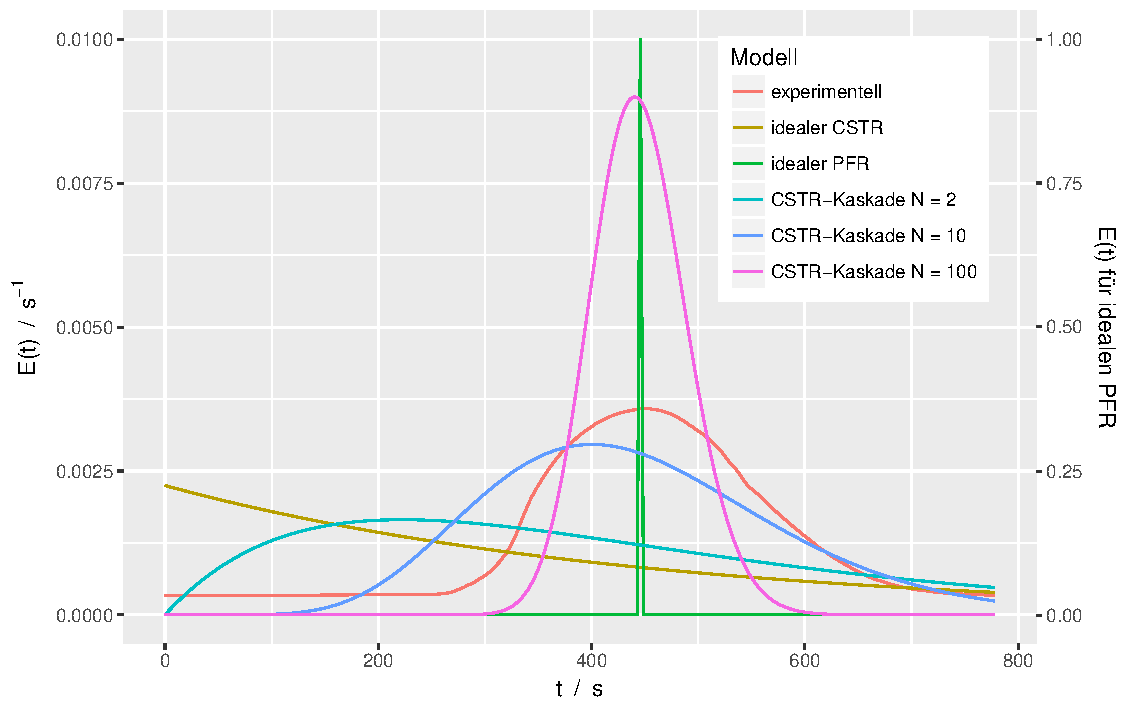
\includegraphics[width=1\textwidth]{Graphics/E_vergleich.pdf}
\caption[Vergleich Verweilzeitdichten]{Vergleich zwischen idealer und experimenteller Verweilzeitdichte}
\label{dichte_vergleich}
\end{figure}
\noindent

\begin{figure}[H]
\centering
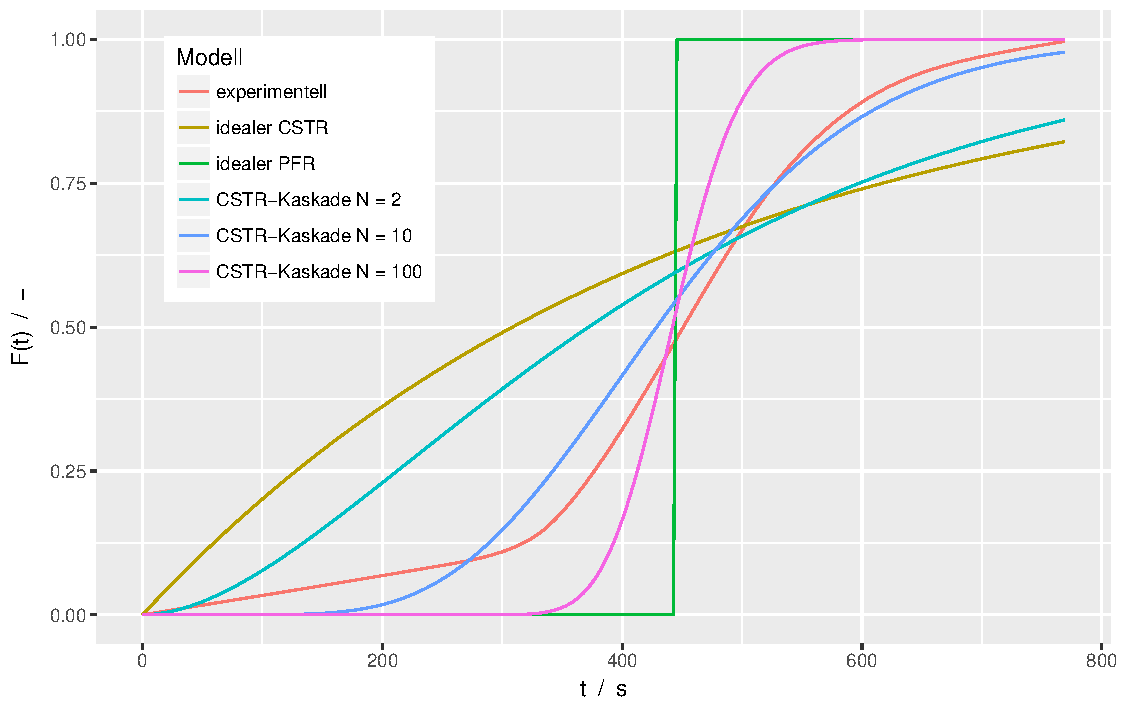
\includegraphics[width=1\textwidth]{Graphics/F_vergleich.pdf}
\caption[Vergleich Verweilzeitsummen]{Vergleich zwischen idealer und experimenteller Verweilzeitsummenverteilung}
\label{summe_vergleich}
\end{figure}
\noindent
\\
\\
Betrachtet man nun exemplarisch Versuch $#$3 (ohne Füllkörper, Pulsmarkierung, 13\,$\frac{\text{ml}}{\text{min}}$ in Abbildung \ref{dichte_vergleich} erkennt man für die Verweilzeitdichteverteilung, dass das oben beschriebene Verhalten der Rührkesselkaskade mit steigender Anzahl an Rührkesseln dem Verhalten des PFRs immer ähnlicher wird. Zudem ist die Pfropfenströmung im PFR am engen Peak der Kurve gut erkennbar, da die hypothetische Konzentration an Tracer zu dem Zeitpunkt detektiert wird zu dem das Volumenelement den Reaktor durchlaufen hat und keine Rückvermischung auftritt. Die Abweichung der aus den Messdaten kalkulierten Verweilzeitverteilung im Realfall von den idealen Fällen lässt sich auf Strömungs-Nichtidealitäten wie Totzonen, Bypassströmungen und Kanalbildung, zurück führen, wobei die Kanalbildung in diesem Fall einen Bereich im Reaktor bezeichnet in welchem die Stromfäden einer Kurve folgen die ein schnelleres Durchlaufen des Reaktors zur Folge haben. An dieser Stelle kann ebenfalls erwähnt werden, dass durch das Aufwickeln des Rohrreaktors der '" Dean-Effekt '" zum Tragen kommt [Quelle]. Durch das Aufwickeln spielen Zentrifugalkräfte eine Rolle, welche durch Geschwindigkeitsdifferenzen im Querschnitt des Rohres variieren diese Zentrifugalkräfte und erzeugen Wirbel, sogenannte "Dean-Wirbel". Diese Wirbel verursachen eine axiale und radiale Durchmischung an der Stelle ihrer Entstehung und beeinflussen folglich die hydraulische Verweilzeit im Reaktor und die Konzentration welche am Ausgang gemessen werden kann. 
\\
\\
Eine weitere mögliche Ursache für die Nicht-Idealitäten bzw. Differenz der realen und theoretischen VWZ-Verteilungen liegt in der Pulsation des Förderstroms, wodurch das Messsignal verfälscht wird bzw. ein Volumenelement mit einer bestimmten Konzentration im Takt der Pumpge gefördert wird und somit beim Messen der Konzentration zwischen zwei Stößen der Pumpe eine andere Konzentration detektiert wird. 
\\
\\
Des Weiteren ist bei Betrachtung von Abbildungen \ref{dichte_vergleich} und \ref{summe_vergleich} erkennbar, dass von den idealen Verläufen die Rührkesselkaskade mit $N$=10 am Besten in der Lage ist den experimentellen Verlauf zu beschreiben. Sprich, der analysierte Rohrreaktor kann in 10 ideale CSTRs mit gleichem Volumen aufgeteilt werden um dem realen Verhalten des Rohrreaktors am nächsten zu kommen. 





\section{Kompartment- und Dispersionsmodell}

Abweichungen von idealen Strömungsverhältnissen beschreiben mit Compartment model, d.h. mit CSTR am Inlet bzw. am Outlet des PFRs, Volumen des CSTR bestimmen und bestimmen ob sich Großteil oder vernachlässigbarer Anteil wie ein CSTR verhält also axiale Vermischung eine Rolle spielt


\section{Bodenstein Zahl mit Dispersionsmodell}

Im Zuge des Laborpraktikums ist zu prüfen ob die Bodensteinnummer mit dem Dispersionsmodell berechenbar ist. Das Modell trifft für Bodenstein-Zahlen von Bo < 100 zu.
\\
\\
Dabei kann für Wertebereiche von $Bo$  das Verhalten eines Reaktors bzw. die Abweichung vom idealen Verhalten bezüglich dem Verhältnis von Konvektion zu Dispersion, beschrieben werden. Folgende Wertebereiche sind von Relevanz:


\begin{itemize}
    \item Bo < 100 mittlere Abweichung vom idealen Fließverhalten
    \item Bo < 1 starke Abweichung vom idealen Flussverhalten
    \item Bo > 100 geringe Abweichung vom idealen Fließverhalten 
\end{itemize}
\noindent
Grundsätzlichen stehen vier Möglichkeiten zur Verfügung um Bo < 100 zu berechnen, wobei sich diese Möglichkeiten durch die angewandten Randbedingungen unterscheiden. Diese Randbedingungen sind Kombinationen von entweder '"closed'" oder '"open'" Vessel (Kessel, Reaktor) und sind durch das Verhalten eines Reaktanden-Teilchens definiert, wobei beim closed Vessel ein Teilchen einer Pfropfenströmung folgt und den betrachteten Reaktorteil nur einmal passieren kann und beim opoen Vessel das betrachtete Teilchen den Reaktorteil mehrmals passieren kann und keine Pfropfenströmung sondern ein ähnliches Strömungsverhältnis zum Reaktoraus- bzw. -eingang vorhanden ist. Folgenden Gleichungen beschreiben laut [Skript] die diversen mathematischen Zusammenhänge zur Kalkulation der Bodenstein-Zahl mit den jeweiligen Randbedingungen.

\begin{enumerate}
    \item Closed-Closed Vessel
    \begin{equation*}
        Bo_{cc} = \left(\frac{1}{\sigma_{\theta}^2 - 1}\right) + \sqrt{\left( \frac{1}{\sigma_{\theta}^2 - 1 \right) + \left( \frac{2}{\sigma_{\theta}} - 2 \right)}
    \end{equation*}
    
    \item Open-Open Vessel
    \begin{equation*}
        Bo_{oo} = \frac{1}{\sigma_{\theta}^2} + \sqrt{\left(\frac{1}{\sigma_{\theta}^2}\right)^2 + \left(\frac{8}{\sigma_{\theta}^2}\right)}
    \end{equation*}
\end{enumerate}
\noindent
In Tabelle \ref{tab:BodensteinDispersion} sind die berechneten Bodenstein-Zahlen zusammengefasst, wobei $Bo$ ohne Index der Kalkulation mit der normierten Standardabweichung $\sigma_{\theta}^2$ entspricht. Als Randbedingungen werden closed-closed (Index $cc$) und open-open (Index $oo$ gewählt, da $oo$ laut Literatur \cite{Skript_2018}, \cite{fogler1999elements} am häufigsten dazu verwendet wird experimentelle Verläufe auszuwerten und die Auswertung mit $cc$ der Bodenstein-Zahl aus der Standardabweichung am nächsten kommt. Daher ist ersichtlich, dass die betrachteten Rohrreaktoren mit der $cc$ Randbedingung am Besten beschreibbar sind und eine Pfropfenströmung am Reaktorein- und -ausgang anzunehmen ist.


\begin{table}[H]
\centering
\caption{Berechnte Bodenstein-Zahlen mit unterschiedlichen Randbedingungen}
\begin{tabular}{cccc}
\toprule 
Experiment $\#$ & $Bo$ & $Bo_{cc}$ & $Bo_{oo}$\\
\midrule
1 & 16,35 & 15,29 & 19,68 \\
2 & 19,26 & 18,21 & 22,66 \\
3 & 20,09 & 19,04 & 23,51 \\
4 & 28,77 & 27,73 & 32,33 \\
5 & 22,06 & 21,02 & 25,52 \\
6 & 31,98 & 30,94 & 35,57 \\
7 & 57,06 & 56,05 & 60,82 \\
8 & 48,80 & 47,78 & 52,52 \\
9 & 44,29 & 43,27 & 47,98 \\
10 & 38,40 & 37,38 & 42,06 \\
11 & 66,09 & 65,07 & 69,87 \\
12 & 87,71 & 86,70 & 91,54 \\
\bottomrule
\end{tabular}
\label{tab:BodensteinDispersion}
\end{table}
\noindent



\section{Reaktion; Umsatz Berechnung aus Verweilzeitverhalten}

Würde theoretisch eine Reaktion im Strömungsrohr ausgeführt werden, so beeinflusst das Verweilzeitverhalten des Reaktors den Umsatz der Reaktion im Sinne der mittleren Verweilzeit und dem  Strömungsverhalten durch Nicht-Idealitäten (Bypass, Totvolumen). Die Berechnung des Umsatzes hängt von der verwendeten Methode ab (Puls- oder Stufenfunktion), da sich die Dichtevereteilung auf eine andere Weise berechnen lässt. Als Reaktion mit weitgehend gut erforschter Kinetik wird die Veresterung von Essigsäure $CH_3COOH$ mit Methanol $CH_3OH$ zu Essigsäuremethylester $CH_3COOCH_3$ und Wasser $H_2O$ gewählt, welche laut Literatur \cite{Rolfe1934}, \cite{mandake2013kinetic} einem Geschwindigkeitsgesetz zweiter Ordnung genügt.

\begin{equation*}
 CH_3COOH + CH_3OH \rightleftharpoons CH_3COOCH_3 + H_2O 
\end{equation*}
\noindent
Im weiteren Verlauf wird der Einfachheit halber die Reaktion mit folgenden Reaktanden referenziert und aufgrund des geringen Wertes der Reaktionsgeschwindigkeitskonstante der Rückreaktion eine irreversible Reaktion angenommen.

\begin{equation*}
    A + B \rightarrow C + D
\end{equation*}
\noindent
Die Kinetik wurde von Hinshelwood et. al und Mandake et. al \cite{Rolfe1934}, \cite{mandake2013kinetic} erforscht und kann für 308\,K (unkatalysiert) mit der Reaktionsgeschwindigkeitskonstante $k$ = 1,5009 $\cdot  $10$^{-2}$\, $\litre\cdot\mole^{-1}\cdot\s^{-1}$ für die Hinreaktion beschrieben werden. In einem nächsten Schritt muss die Anfangskonzentration $c_{A,0}$ definiert werden, welche im Verhältnis zur gemessenen Konzentration an NaCl-Tracer stehen kann, aber nicht muss, damit die gemessenen Werte der Leitfähigkeit bzw. Konzentration im Experiment für die Ermittlung des realen Umsatzes herangezogen werden können. Damit die Umsätze aber Werte erreichen die gut vergleichbar sind und nicht zu gering sind wird die Anfangskonzentration an Essigsäure $CH_3COOH$ mit $c_{A,0}$ = 2\,$\frac{\text{mol}}{\text{l}}$ definiert und für alle Versuche konstant gehalten. 
\\
\\
Das Geschwindigkeitsgesetz zweiter Ordnung und die Kalkulation des Umsatzes für den realen und idealen Fall ist im Folgenden dargestellt.

\begin{align}
&\biggl(\frac{\bar{c}_A}{c_{A,0}}\biggr)_{real} = \int_{0}^{\infty} \biggl(\frac{{c}_A}{c_{A,0}}\biggr)_{ideal} \cdot E(t)\cdot dt = (1-X_{real})\\
&\text{mit } \biggl(\frac{{c}_A}{c_{A,0}}\biggr)_{ideal} = \frac{1}{1+k\cdot c_{A,0}\cdot \bar{t}}\notag
\end{align}

Wird das Integral numerisch gelöst ergibt sich Gleichung \ref{gl_Umsatz}. Für die Reaktion ergibt sich somit folgender Umsatz:

\begin{align}
& (1-X_{real}) = \sum \biggl(\frac{{c}_A}{c_{A,0}}\biggr)_{ideal} \cdot E(t)\cdot \Delta t\\ \label{gl_Umsatz}
& (1-X_{real}) = \sum \biggl(\frac{{c}_A}{c_{A,0}}\biggr)_{ideal} \cdot E(t)\cdot \Delta t\\ \notag
& X_{real} = 1- \approx \notag
\end{align}

Um die Nicht-Idealitäten der untersuchten Reaktoren mit dem Umsatz in Verbindung zu bringen werden die Versuche mit einem Durchfluss von XXX\,$\frac{\text{ml}}{\text{min}}$ für die Reaktoren mit und ohne Füllkörper gewählt.
\\
\\
Die nach obigem Algorithmus ermittelten Umsätze sind in Tabelle XXX gelistet.

\begin{table}[H]
\centering
\caption{Umsätze der Veresterungsreaktion ideal und real}
\begin{tabular}{ccc}
\toprule 
Reaktor $\&$ Durchfluss & $c_{A,0}$ in $\frac{\text{mol}}{\text{l}}$ & $X_{A,ideal}$ & $X_{A,real}$\\
\midrule
1 $\&$ X\,$\frac{\text{ml}}{\text{min}}$ & XXX & XXX & XXX\\
\bottomrule
\end{tabular}
\label{tab:umsatz}
\end{table}
\noindent
asdf





\chapter{Conclusio}


Dean Effect!





\newpage
\pagenumbering{arabic}

\newpage
 \pagenumbering{Roman}
\setcounter{page}{2}

\newpage
\listoffigures

\newpage
\listoftables


\newpage

%\bibliography{quellen} 
%\bibliographystyle{ieeetr}
%\addcontentsline{toc}{chapter}{Literaturverzeichnis}
\bibliographystyle{unsrtdin}
\addcontentsline{toc}{chapter}{Literaturverzeichnis} 
\bibliography{Quelle_CRT_2}
\printbibliography


\newpage
\chapter*{Symbolverzeichnis}
\addcontentsline{toc}{chapter}{Symbolverzeichnis}



\begin{table}[H]
\renewcommand{\arraystretch}{1.5}
\setlength{\tabcolsep}{9mm}
\begin{tabular}{llr}
\textbf{Symbol} & \textbf{Bedeutung} & \textbf{Einheit}\\
$\dot{V}$ & Volumenstrom & m$^3$s$^{-1}$\\
$p$ & Druck & Pa\\
$\rho$ & Dichte & kg m$^{-3}$\\
$g$ & Erdbeschleunigung & m s$^{-2}$\\
$h, H$ & Höhe & m\\
$m$ & Masse & kg\\
$m\%$ & Massenprozent & - (\%)\\
$\Delta m$ & Massendifferenz & kg\\
$d$ & Durchmesser & m\\
$d_{32}$ & Sauter-Durchmesser & m\\
$S_V$ & spezifische Oberfläche & m$^{-1}$\\
$Q$ & Verteilungssumme & -\\
$\epsilon$ & Porosität & -\\
$Ar$ & Archimedes-Zahl & -\\
$\eta$ & dynamische Viskosität & Pa s\\
$v$ & Geschwindigkeit & m s$^{-1}$\\
$v$ & Leerrohr-Geschwindigkeit & m s$^{-1}$\\
$Re$ & Reynolds-Zahl & -\\
\end{tabular}
\end{table}

\begin{table}[H]
\renewcommand{\arraystretch}{1.5}
\setlength{\tabcolsep}{9mm}
\begin{tabular}{llr}
\textbf{Indizes} & \textbf{Bedeutung} &\\
$i$ & auf Messpunkt bezogen (z.B. Maschendurchmesser Sieb)\\
$gew$ & (nach Masse) gewichtet\\
$gem$ & gemittelt\\
$min$ & minimal\\
$Bett$ & Schüttungsbett\\
$sch$ & Schüttung\\
$p$ & Partikel\\
$f$ & Fluid\\
$L$ & Lockerungspunkt\\
$R$ & Rohr\\
$Anlage$ & Anlage\\
$b,0$ & Blase, am Gasverteiler\\
$b,m$ & Blase, maximal\\
$b$ & Blase\\
\end{tabular}
\end{table}

\newpage



\appendix
\chapter*{Anhang}
\addcontentsline{toc}{chapter}{Anhang}


\end{document}
